\documentclass[a4paper, 10pt, oneside]{article} 

\usepackage[T1]{fontenc}
\usepackage[utf8]{inputenc}

\usepackage[magyar]{babel}
\usepackage{graphicx}
\usepackage{subfig}
\usepackage{multirow}
\usepackage{amsmath, amssymb, physics, verbatim}

\usepackage{hyperref}
\usepackage{float}
\usepackage[font=footnotesize]{caption}
\usepackage[a4paper,
			bindingoffset=0.3in,
            left=0.30in,
            right=0.30in,
            top=0.66in,
            bottom=0.5in,
            footskip=.25in]{geometry}

% Ez feltolja a címet
\usepackage{titling}
\setlength{\droptitle}{-2cm}
% Ez meg átváltja a fontot
%\usepackage{newtxtext}

\title{ Találd fel magad! } 
\author{\textit{Farkas Zsombor, Gillich Ádám, Győrfi Szabolcs, Milbik Csongor László}}
\date{\today} 

%-------------------------------------------------------------------------------------------
\begin{document}

\maketitle

\section{Mérés célja}
	Vezetéken átfolyó áram nagyságának meghatározása annak hőhatása alapján, kihasználva a vezetékben fellépő hőtágulás jelenségét.

%-------------------------------------------------------------------------------------------
\section{Mérés elméleti összeállítása}
Az alábbi ábra szemlélteti a mérési elrendezés alapvető struktúráját.
	\begin{figure}[H]
		\centering
		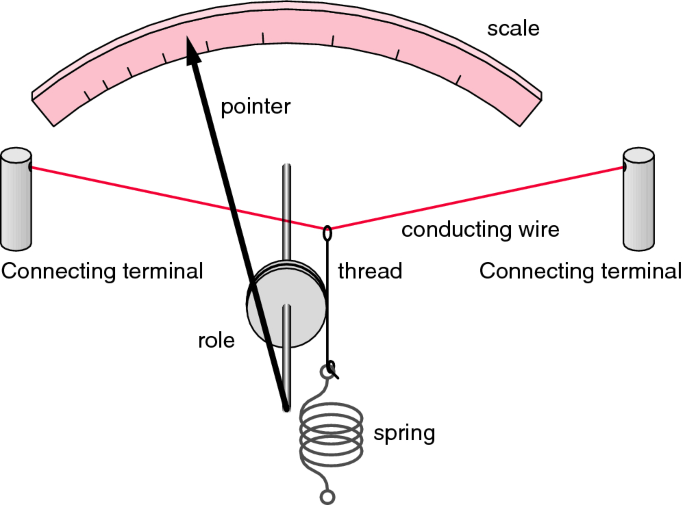
\includegraphics[scale=0.25]{Pictures/tervrajz.png}
		\caption{Mérés összeállításának tervrajza \cite{Terv}}
	\end{figure}

%-------------------------------------------------------------------------------------------
\section{Mérés rövid leírása}

	Az ábrának megfelelően vékony vezetéket feszítünk ki, amin áram folyik át, mely felmelegíti a vezetéket a Joule-hő keletkezésének hatására. Azonban a vezeték le is ad 
	hőt a környezetének mind hőátadás, mind pedig hősugárzás keretében. Mivel az időegység alatt leadott hő mennyisége nő a vezeték 
	hőmérsékletének növekedésével, ezért lesz egy olyan egyensúlyi hőmérséklet, ahol a felvett és a leadott hőteljesítmény egyenlő, ezen a 
	hőmérsékleten marad a vezeték (most és a továbbiakban is tekintsünk el a környezet felmelegedésétől). 
	A hőmérséklet-növekedés hatására a vezeték kitágul, így megváltozik a hossza, így a ráakasztott kötél 
	lejjebb \textqq{esik}, megmozgatva a csigát, amin található mutató így kimozdul. Ez a szögelfordulás a hőtágulás okozta kis elmozdulást már felnagyítja, így ez közvetlenül mérhető mennyiség. Elméleti (modell alapján számoljuk) és tapasztalati (empirikus kalibráció) úton is meg tudunk feleltetni adott szögelfordulást adott áramerősségnek.

%-------------------------------------------------------------------------------------------
\section{Vizsgálati módszer}
A méréshez szükséges eszközök:
\begin{itemize}
	\item Tápegység
	\item Multiméter
	\item Állítható ellenállás
	\item Kábelek, krokodil csipesz
\end{itemize}

Fontos, hogy olyan tápegység kell, amin a feszültség és így az áramerősség állítható. Állítható ellenállás, 
lehet egy tolóellenállás, vagy esetünkben egy potméter, ez azért kell, hogy tápegység leadott áramerősség 
minimuma alatt tudjunk adatokat mérni. Krokodil csipesz pedig a műszer bekötéséhez szükséges.\\

A mérés innentől triviális, a rendszerbe áramot kapcsolunk, majd megnézzük mennyit mozdul a mutató, és milyen értékeket mutat a multiméter. Ezt háromszor megismételjük áramerősségenként.\footnote{Meg kell jegyeznem, 
hogyha állítható tápegység nem áll rendelkezésre, akkor megfeleő számú (1 – 6+) ceruzaelem sorbakötésével, 
szintén megismételhető a kísérlet.}\\

%-------------------------------------------------------------------------------------------
\section{Mérés gyakorlati összeállítása} 

	\begin{figure}[H]
	 	\centering
		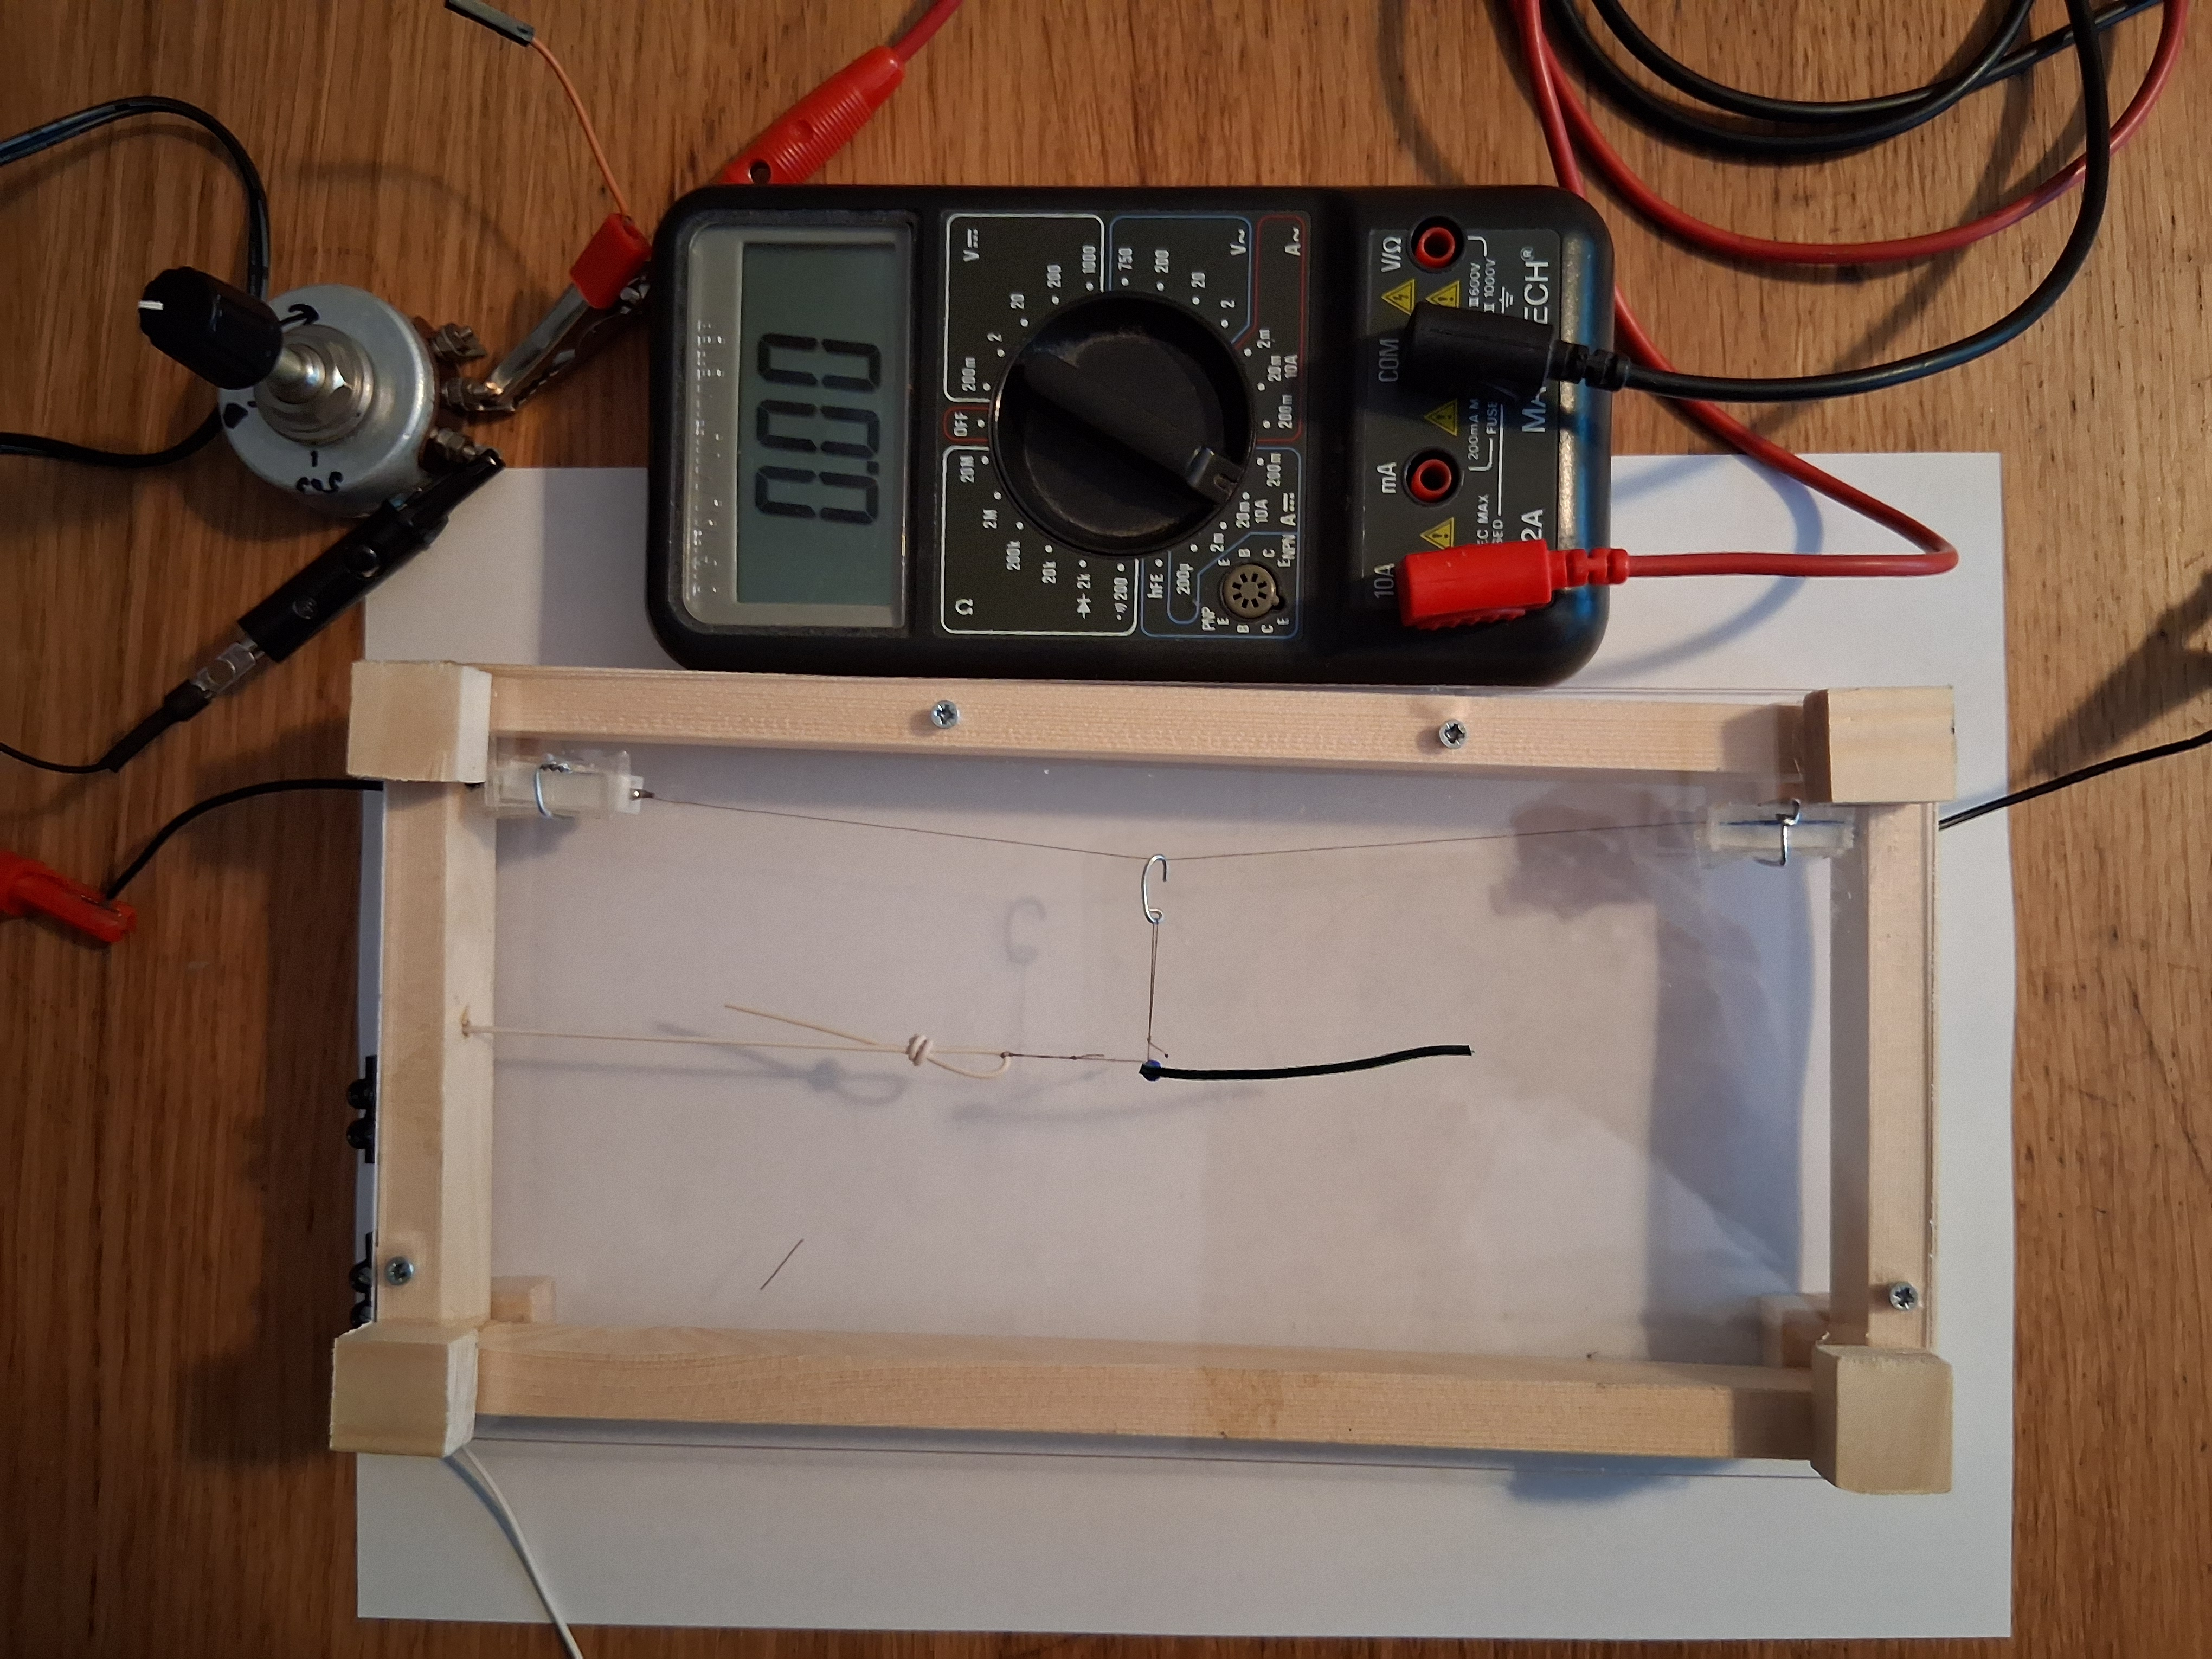
\includegraphics[scale=0.1]{Pictures/műszer_kistotal.jpg}
		\caption{Mérőeszközről készült kép}
	\end{figure}

	Az általunk összerakott mérőeszköz követi a tervrajz mintáját. Vezetéknek nikrómot használtunk, csigának 
	pedig egy gombostűt. Továbbá a rugó helyett egy gumiszál került be.

	\begin{figure}[H]
	 	\centering
		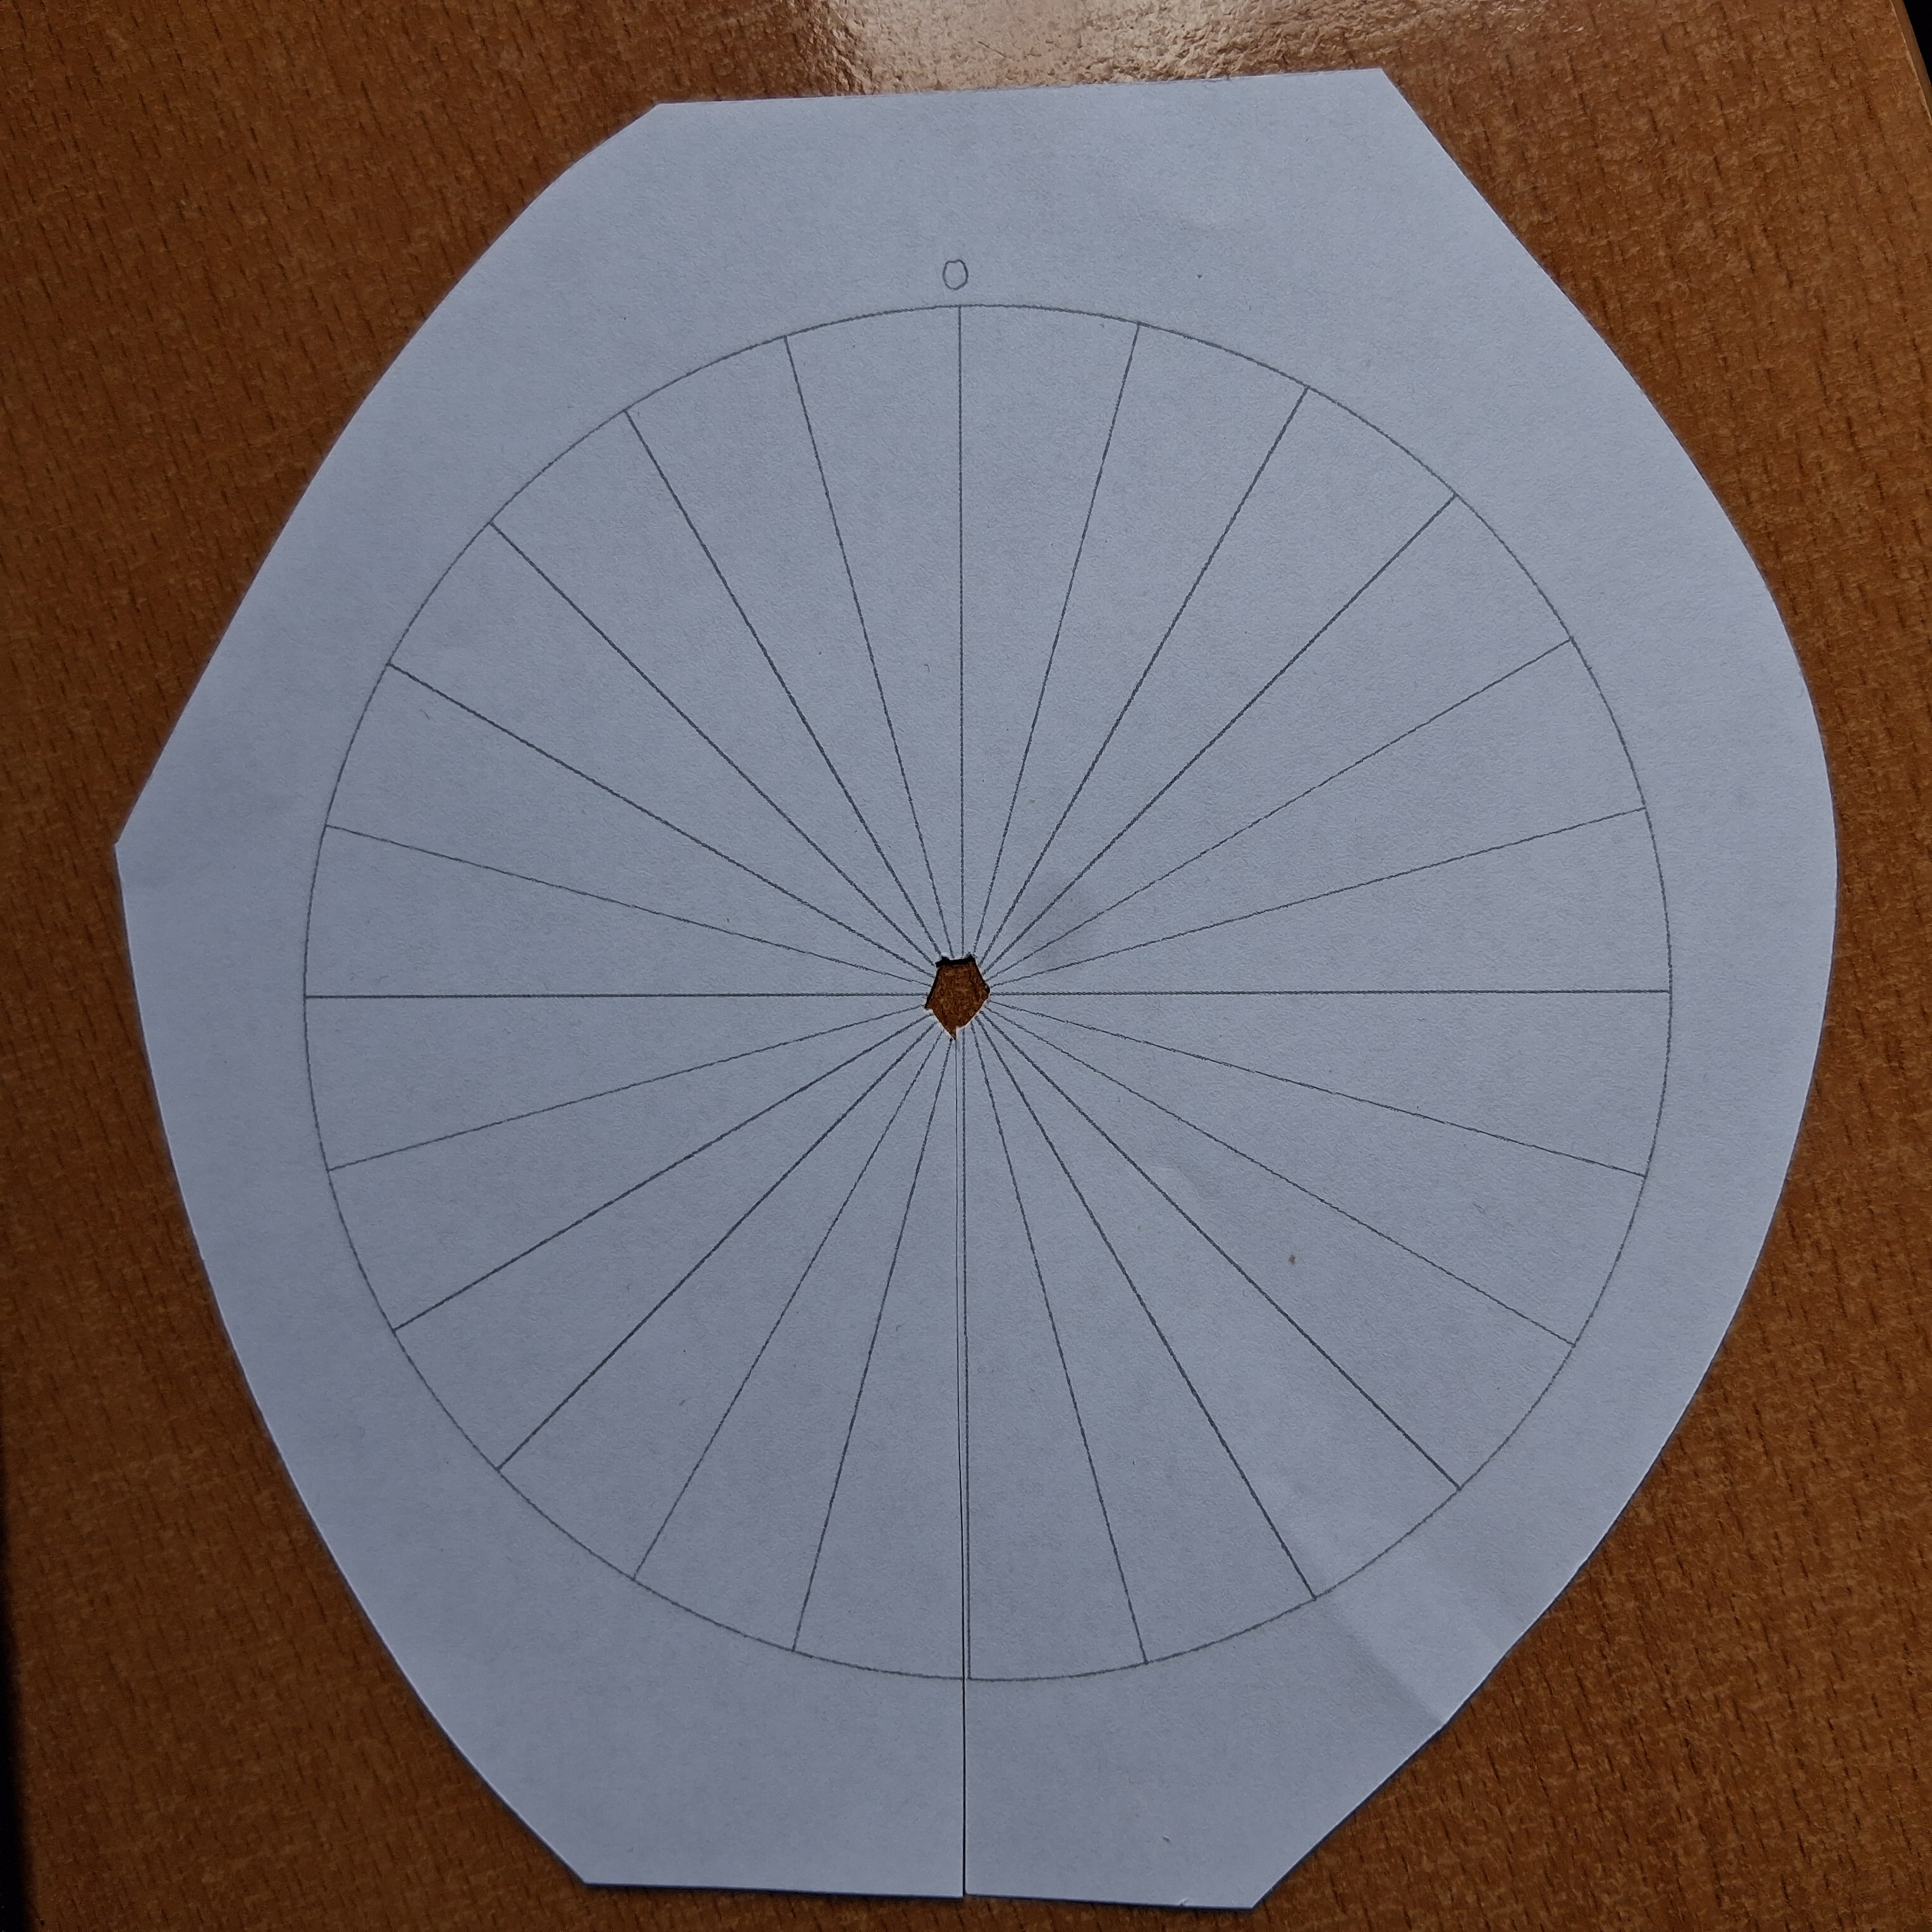
\includegraphics[scale=0.06]{Pictures/szamlap.jpg}
		\caption{Mérőeszköz számlapja}
	\end{figure}

	A műszerhez nyomtatott, majd méretrevágott számlapot használtunk az adatok leolvasására. A számlap
	közepéből radiálisan $15^\circ$-ként jönnek vonalak.

%-------------------------------------------------------------------------------------------
\section{Mérőeszköz elmélete}

\subsection*{A vezeték megnyúlása}
	A vezeték kétféleképpen is lead hőt. A hőátadásra a Newton-féle lehűlési törvényt alkalmazzuk 
	közelítésnek, miszerint: 

	\[ \frac{dQ}{dt}=-NA(T-T_k), \]

	\indent ahol $N$ a hőátadási együttható, $A$ a vezeték 
	felülete, $T$ a vezeték hőmérséklete, $T_k$ a környezet hőmérséklete. Továbbá a hősugárzás sem lesz 
	elhanyagolható, így az összes leadott hő:
	
	\[ \boxed{\frac{dQ}{dt}=NA(T-T_k)+\epsilon A \sigma(T^4-T_k^4)}\ , \]

	\indent ahol $\epsilon$ az emissziós tényező, 
	esetünkben legyen 0.8 \cite{epsilon}, $\sigma$ a Stefan-Boltzman-állandó, ami 
	$5.67^{-8} \frac{W}{m^2 K^4}$. $N$ eléggé függ a mérési viszonyoktól és a vezeték alakjától, 
	de most közelítve legyen konstans $35 \frac{W}{m^2 K}$. A felvett hő a Joule hőből származik, ami 
	$\frac{dQ}{dt}=I^2 \cdot R$, ahol $I$ a vezetéken átfolyó áram, $R$ a vezeték ellenállása. Bár az 
	ellenállás értéke is függ a hőmérséklettől, a nikróm ellenállása magas hőmérsékleten is csak kicsit 
	változik \cite{R-T}, ezért legyen a továbbiakban konstans.\\ 
	\indent Közelítsük a rúd megnyúlását úgy, hogy: 

	\[ l=l_0e^{\alpha(T-T_k)}, \]

	\indent ahol $l$ a vezeték hossza, $l_0$ a vezeték eredeti hossza, $\alpha$ a 
	hőtágulási együttható (esetünkben most legyen konstans $14 \cdot 10^{-6}\ 1/K$, de egyébként ez is 
	hőmérsékletfüggő). A vezeték sugara hasonlóan tágul:
	
	\[ r=r_0e^{\alpha(T-T_k)}, \]

	ahol $r$ a vezeték sugara, $r_0$ a vezeték eredeti sugara. Így a vezeték levegővel érintkező felülete:
	
	\[ A=2\pi r l=2\pi r_0l_0e^{2\alpha(T-T_k)}. \]

	\noindent Továbbá ki lehet fejezni a $T-T_k$-t a vezeték hosszával $T-T_k=\frac{ln(\frac{l}{l_0})}{\alpha}$.\\ 
	\indent Az eddigi egyenleteket összerakva egyensúlyban:
	\[
		\boxed{
			N \cdot 2\pi r_0l_0 \bigg(\frac{l}{l_0}\bigg)^2 \cdot
		    \frac{ln\frac{l}{l_0}}{\alpha}
		    +2\pi r_0l_0 \bigg(\frac{l}{l_0}\bigg)^2 \cdot\epsilon\sigma\left[\Bigg(\frac{ln\frac{l}{l_0}}{\alpha}-T_k\Bigg)^4-T_k^4\right] =I^2R} \ .
	\]
	Innen már numerikusan számolható a vezeték megnyúlt hossza.

\subsection*{A csiga elfordulása}
	Nézzük a csiga megmozgatásának geometriáját. 

	\begin{figure}[H]
		\centering
		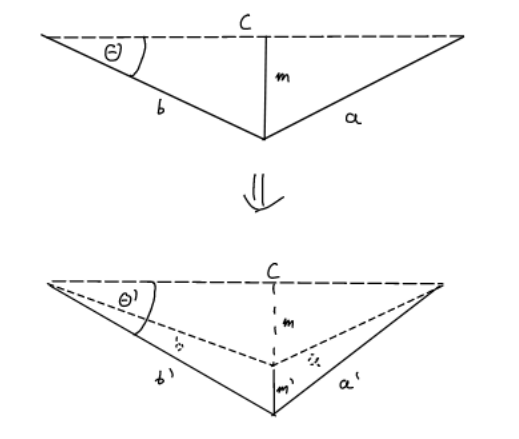
\includegraphics[scale=0.5]{Pictures/geometria.png}
		\caption{A vezeték megnyúlásának geometriája}
	\end{figure}


\noindent Koszinusztétel alapján:
\[ \cos\Theta=\frac{b^2+c^2-a^2}{2bc}, \]
továbbá:
\[ m=b\sin\Theta=b\sqrt{1-\cos^2\Theta}. \]
A magasság a $c$ oldalt két részre osztja, legyen a $b$ oldali rész $c_b=b\cos\Theta$. Megnyúlás után felírható
 megint csak a koszinusztétel: $\cos\Theta '=\frac{b'^2+c^2-a'^2}{2b'c}$, továbbá $\cos\Theta'=\frac{c_b}{b'}$. 
 A kettőt összerakva 
\[ 2c_b=\frac{b'^2+c^2-a'^2}{c}. \]
 Mivel a vezeték hossza $a'+b'=l$, ezért egyértelműen 
 meghatározható $a', b'$. Innen $m'=\sqrt{b'^2-c_b^2}$. Így a csiga forgása:

\[ \boxed{\Delta m=\phi (d/2)} \]

\indent ahol $\Delta m=m'-m$, $d$ a csiga átmérője, $\phi$ a csiga szögelfordulása.

\subsection*{A program}

\begin{figure}[H]
	\centering
	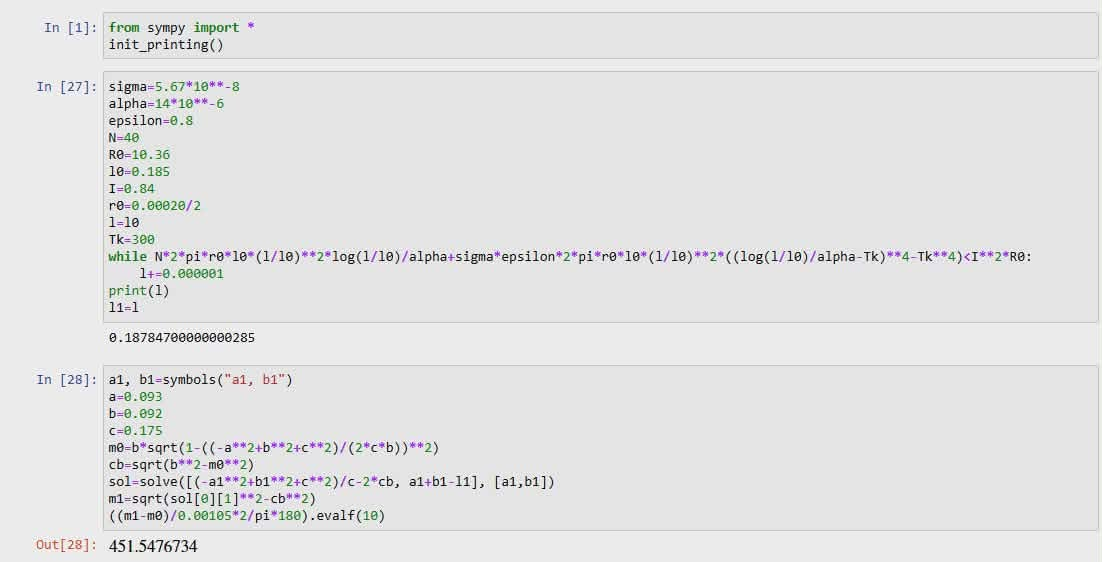
\includegraphics[scale=0.44]{Pictures/szabi_kod_javitott.jpg}
	\caption{Az eredményeket számláló numerikus program}
\end{figure}

%-------------------------------------------------------------------------------------------
\section{Mérési adatok, kiértékelés}

\begin{table}[H]
	\centering
	\begin{tabular}{|c|c|}
		\hline
		a [cm]     & 9.26794   \\ \hline
		b [cm]     & 9.16794   \\ \hline
		c [cm]     & 17.5  \\ \hline
		d [mm]     & 1.05  \\ \hline
		$r_0$ [mm] & 0.12   \\ \hline
		R [$\Omega$] & 10.36 \\ \hline
	\end{tabular}
	\caption{Rendszerre jellemző adatok, hibahatáron belül optimalizálva}
\end{table}

\begin{figure}[H]
	\centering
	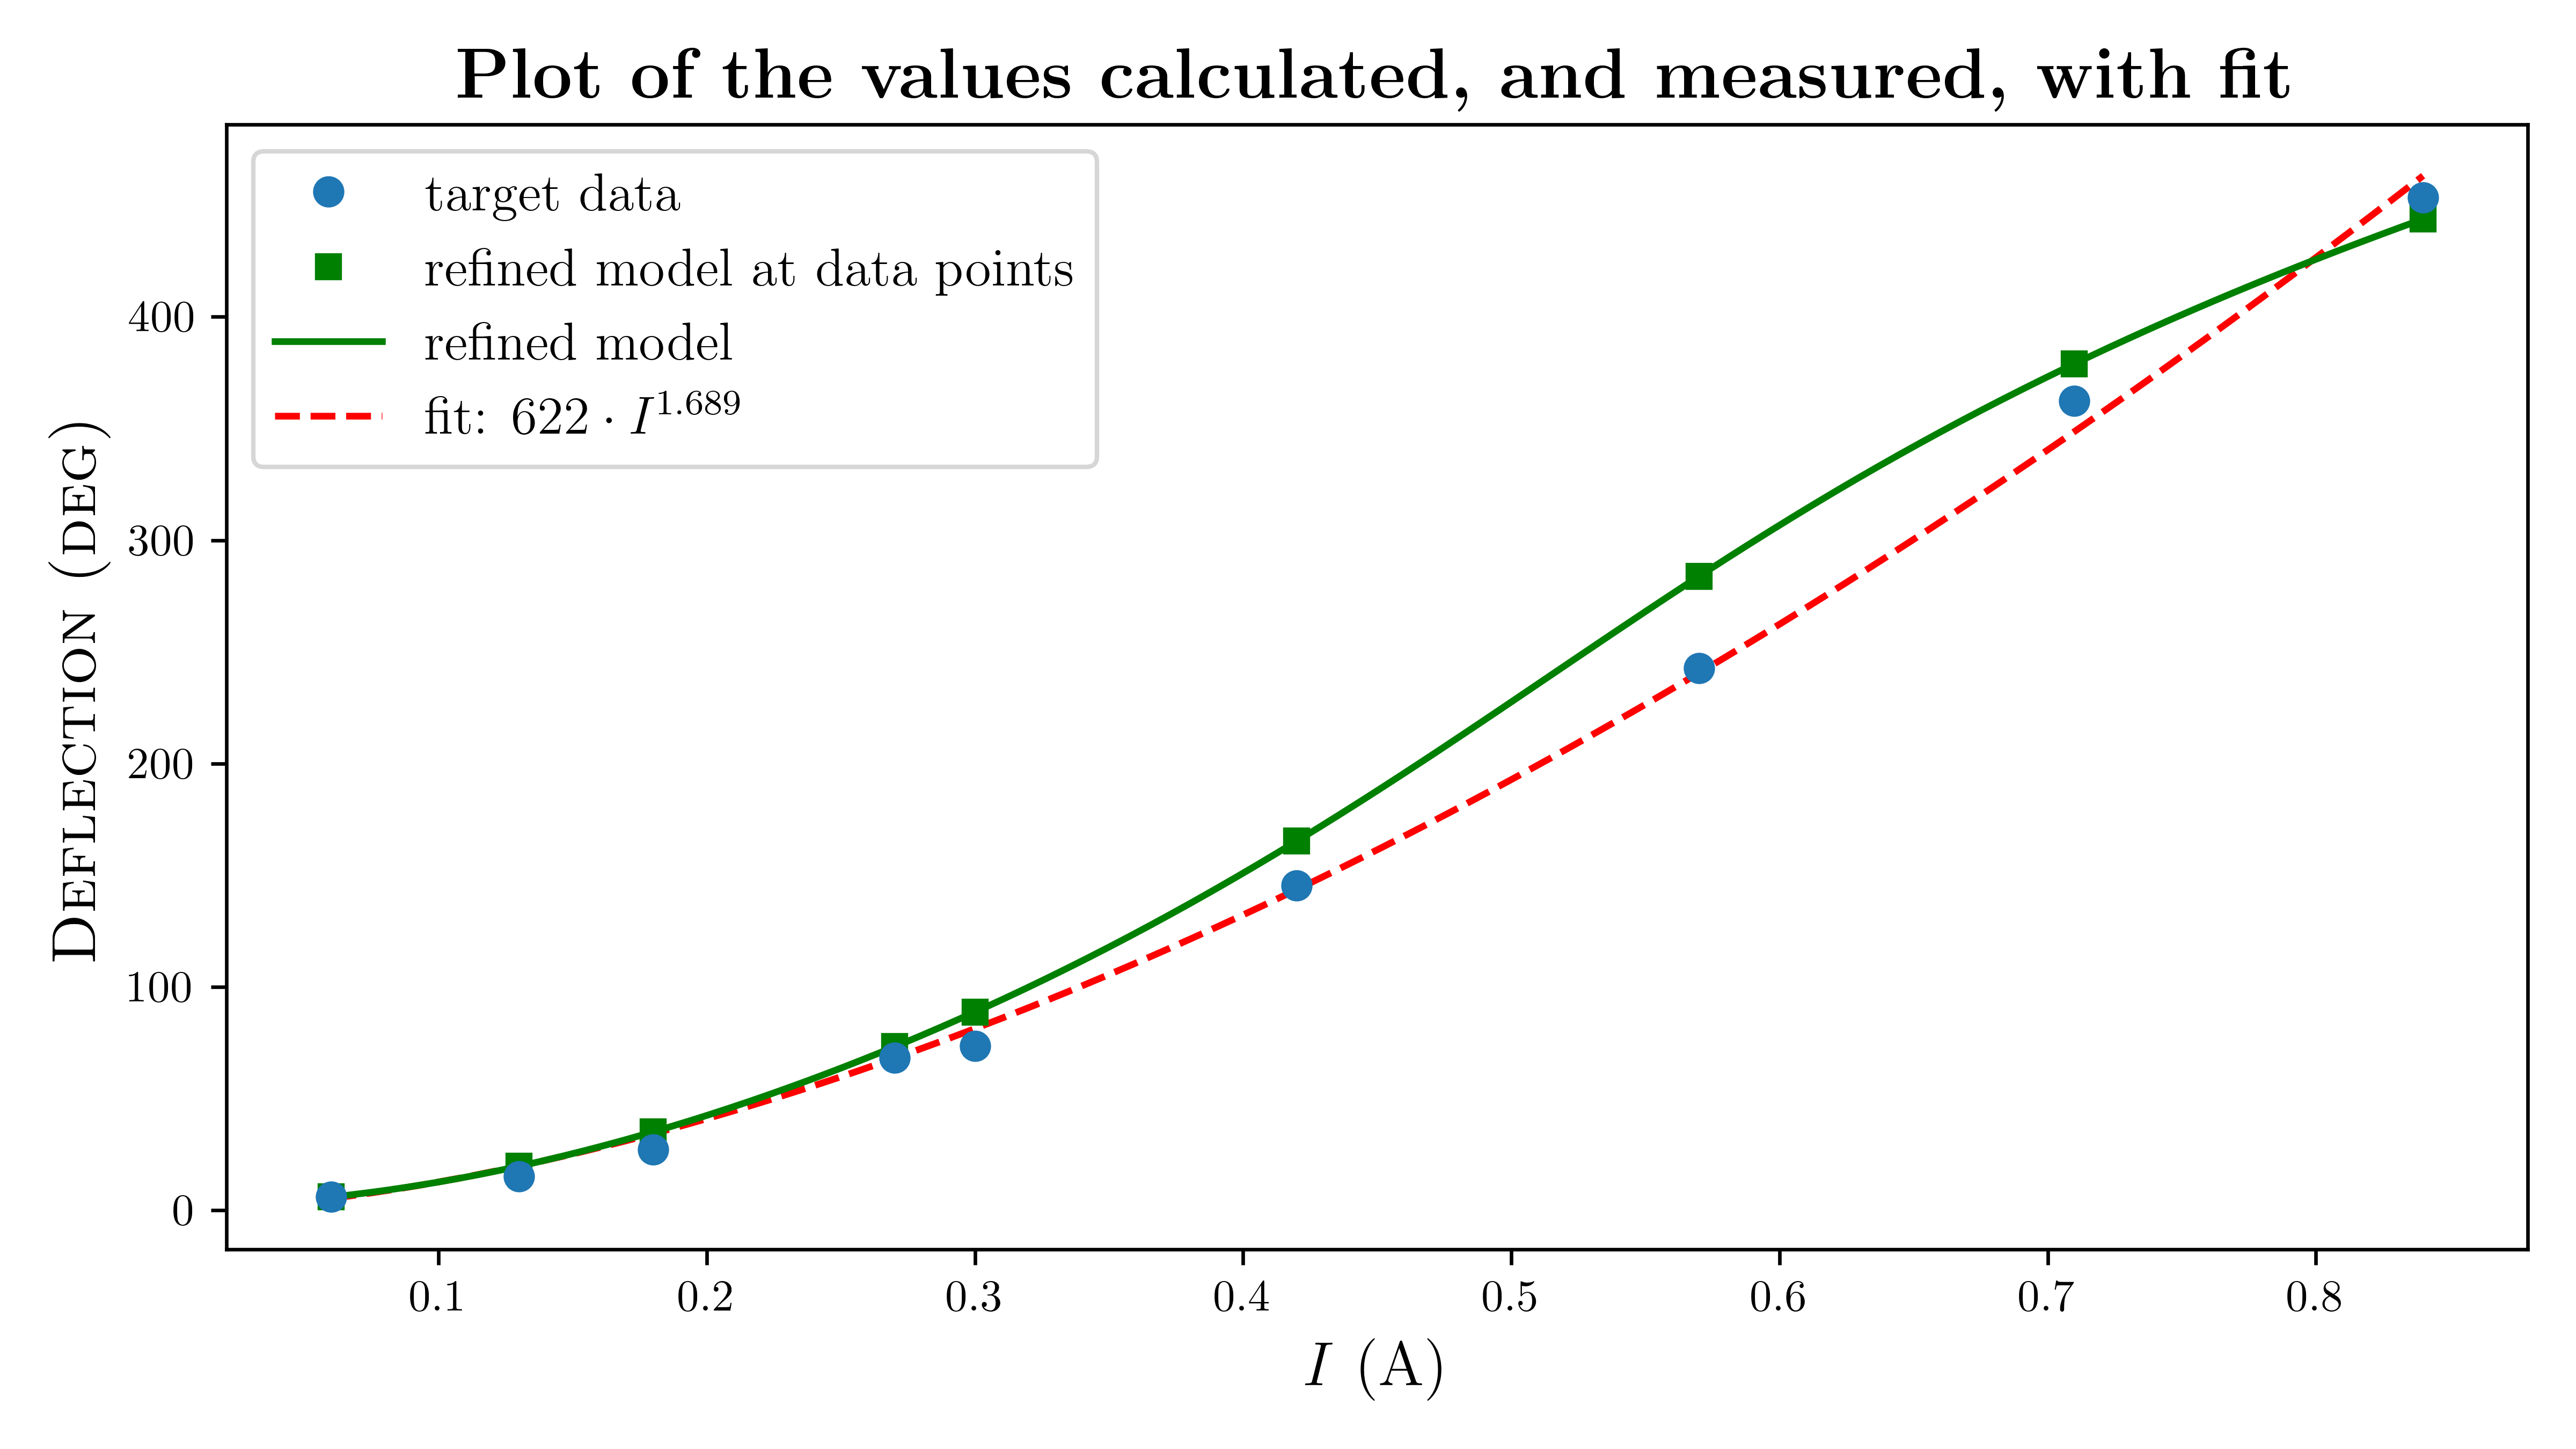
\includegraphics[scale=0.7]{Pictures/plot_javitott.png}
	\caption{Ábra a számolt és mért adatokról, illesztett görbével}
	\label{abra6}
\end{figure}

\footnotetext[2]{{\Aref{table2} táblázat különbség oszlopa az Átlag és a Számolt szögelfordulást veti össze.}}

\begin{table}[H]
\centering
	\begin{tabular}{|c|ccc|c|c|c|}
		\hline
		Áramerősség [A] & \multicolumn{3}{c|}{Mért szögelfordulás [°]} & Átlag [°] & Számolt szögelfordulás [°] & Különbségek [°] \\ \hline
		0.06 & \multicolumn{1}{c|}{7}   & \multicolumn{1}{c|}{5}   & 6   & 6      &   5.990 &   0.010 \\ \hline
		0.13 & \multicolumn{1}{c|}{15}  & \multicolumn{1}{c|}{15}  & 16  & 15.33  &  19.777 &  -4.447 \\ \hline
		0.18 & \multicolumn{1}{c|}{31}  & \multicolumn{1}{c|}{30}  & 21  & 27.33  &  35.164 &  -7.834 \\ \hline
		0.27 & \multicolumn{1}{c|}{72}  & \multicolumn{1}{c|}{68}  & 65  & 68.33  &  73.259 &  -4.929 \\ \hline
		0.3  & \multicolumn{1}{c|}{75}  & \multicolumn{1}{c|}{71}  & 75  & 73.67  &  88.803 & -15.133 \\ \hline
		0.42 & \multicolumn{1}{c|}{142} & \multicolumn{1}{c|}{144} & 150 & 145.33 & 165.327 & -19.997 \\ \hline
		0.57 & \multicolumn{1}{c|}{240} & \multicolumn{1}{c|}{247} & 241 & 242.67 & 283.874 & -41.204 \\ \hline
		0.71 & \multicolumn{1}{c|}{362} & \multicolumn{1}{c|}{360} & 365 & 362.33 & 379.013 & -16.683 \\ \hline
		0.84 & \multicolumn{1}{c|}{458} & \multicolumn{1}{c|}{450} & 452 & 453.33 & 443.815 &   9.515 \\ \hline
	\end{tabular}
	\caption{A kimért szögelfordulások az áramerősség függvényében, és a hozzá számolt értékek az elméletből.}
	\label{table2}
\end{table}

Mérés közben azt tapasztaltuk, hogy a választott $0$ ponttól indulva $\Delta \phi$ kitérés konzisztens, azaz adott áramerősséghez ugyanolyan szögelfordulásokat kaptunk többszöri mérés során is, viszont 
kikapcsolás után a mutató nem tér vissza pontosan a $0$ pontba. Ezért minden egyes áramerősség értéknél, 
igazítanunk kellett a $0$-t.

%-------------------------------------------------------------------------------------------
\section{Diszkusszió}

Az elméleti számolás és a gyakorlat között a nagyobb áramerősségeknél nagy az eltérés. Ez azért lehet, 
mert sok dolog, pl. a huzal ellenállása kicsit hőmérsékletfüggő, amit konstansnak vettünk, és nagy áramerősségeknél 
már a vezeték 
is magas hőmérsékletű lesz. Ezeket a hibákat kiküszöbölhetné hogyha ezen mennyiségek hőmérsékletfüggését beépítenénk 
az elméleti modellbe. Továbbá a gumi általi húzóerejének változását nem vettük figyelembe, ami a vezeték nagyobb 
megnyúlásánál 
egyre kisebb lesz, így kevésbé húzza ki azt. A kiküszöbölés lehetséges módja itt is a bonyolultabb számolás lehetne. 
Fontos megemlíteni még azt is, hogy a csiga sugara kicsi, 
így ennek meghatározásánál kis abszolút hiba is nagy relatív hibát eredményezhet.\\

\indent Még pontatlanságot okozhat az, hogy a vezeték nem élesen törik meg, mint egy háromszögnél, hanem hajlik. Amit 
elhanyagoltunk.
Ezen kívül fellép a holtjáték jelensége a csigán fellépő súrlódás miatt. És ez lehet a magyarázata annak amit 
tapasztaltunk mérés közben, azaz hogy minden alkalommal újra kellett kalibrálnunk a 0 viszonyítási pontot.

\subsection*{Méréshatár}

A műszer teljes méréshatára egy körbefordulás, ami nagyjából $0.7\, A$, hogyha ezen túl megyünk akkor a műszer 
mutatója körbefordul, így nem lesz egyértelmű, az hogy hova mutat (pl.: $0.8\, A$-re, vagy $0.3\, A$-ra). Ezen
kívül méréshatárt képez a is, hogy valamennyivel $0.84\, A$ fölött a szál elkezd izzani, és el is pattanhat.

\subsection*{Pontosság}

\subsubsection*{Műszer pontossága}
A műszerrel lehet néhány század ampert mérni, mint az \aref{table2} táblázatból is látszik, és nagyjából, 
kis áramerősségeknél lineárisan. Viszont nagy kitérésekél, már nem lineáris a kitérés, és a hiba sem. Nagy 
áramerősségeknél nagyobb lesz a hiba, és a holtjáték is. Például $360^\circ$-nál tovább azért sem érdemes menni
mert a műszer olyan gyorsan tér ki, hogy $0.84\, A$-nél, $\approx20^\circ$-kal többet is mutat eleinte, majd egy kis idő 
elteltével visszamegy $20^\circ$-t, ahogy beáll az egyen súlyi állapot. Így jön ki \aref{table2} táblázatban
látható $360^\circ+90^\circ \approx 450^\circ$.

\subsubsection*{Elmélet pontossága}

\Aref{abra6} ábrából láthatjuk, hogy az elméletünk nagyobb áramerősségekre jelentősen eltér a mért adatokra illesztett 
függvény alakjától.
De, mint az \aref{table2} táblázat Különbség oszlopából is látszik, az eltérés kis áramok esetén tűrhető. $0.84\, A$-nál 
már elszáll, 
de a műszer méréshatára $0.7\, A$, és addig az elmélet elfogadhatóan követi a tapasztalatot.

\begin{thebibliography}{99}
\bibitem{Terv} \href{https://link.springer.com/chapter/10.1007/978-3-030-02291-4_2}{Terv képe innen van}.
\bibitem{epsilon} \href{https://www.engineeringtoolbox.com/emissivity-coefficients-d_447.html}{Nikróm emissziós tényezője innen van}.
\bibitem{R-T} \href{https://wiretron.com/nichrome-resistance-informational-charts/}{Innen van a Nikróm ellenállásának változása hőmérséklet-változásra}


\end{thebibliography}
\end{document}
